%-----------------------------------
%
\chapter{Assembly}
%
%-----------------------------------

\AY{Different ways to put the above layers together/ordering them. Simulating RASPS and etc can go here?}

\section{Comparison}
\label{sec:assembly_comparison}

\AY{Comparing numerical values. The part that makes this slightly unstraightforward is ensuring that the result is in the desired Boolean representation}

Assumptions:
\begin{itemize}
    \item Function from $\Z\times\Z\to \left\{\begin{bmatrix}
            -1\\\phantom- 1
        \end{bmatrix}, \begin{bmatrix}
            \phantom- 1\\-1
        \end{bmatrix}\right\}$
\end{itemize}

This requires access to $\pm\frac{1}{i+1}$ in some dimensions $2k_0-1,2k_0$. 
        
    First we explain how to simulate a comparison of two count terms $C_1(i)\leq C_2(i)$. Then, we describe how to extend this to %simulate, for sets of indices $X_1$ and $X_2$, the expression \[\sum_{x\in X_1} c_{x} \cdot C_x(i) \leq \sum_{x\in X_2} c_{x} \cdot C_x(i).\]
    compare linear combinations of count terms.
    
    Suppose that we want to compare $C_1$ and $C_2$ in dimensions $2k_1-1,2k_1$ and $2k_2-1,2k_2$, and put the result in dimension $2k_3-1,2k_3$. Initially, the residual stream looks like this:
    \begin{equation*}
    \begin{blockarray}{cccc}
        & & i & \\
        \begin{block}{c[ccc]}
                &  & \vdots &  \\
               2k_0-1 & \cdots & -\frac{1}{i+1} & \cdots \\[6pt]
                2k_0 & \cdots & +\frac{1}{i+1} & \cdots \\
                & & \vdots & \\[6pt]
               2k_1-1 & \cdots & -\frac{C_1(i)}{i+1} & \cdots \\[6pt]
                2k_1 & \cdots & +\frac{C_1(i)}{i+1} & \cdots \\
                & & \vdots & \\
               2k_2-1 & \cdots & -\frac{C_2(i)}{i+1} & \cdots \\[6pt]
                2k_2 & \cdots & +\frac{C_2(i)}{i+1} & \cdots \\
              & & \vdots & \\
               2k_3-1 & \cdots & 0 & \cdots \\[6pt]
                2k_3 & \cdots & 0 & \cdots \\
                & & \vdots & \\
        \end{block}
    \end{blockarray}
    \end{equation*}

    \newcommand{\clipfn}{\operatorname{gtz}}

    We construct a feed-forward layer that computes the function: 
    \[\clipfn(X(i)) = \min\left(\frac{0.5}{i+1},\frac{X(i)}{i+1}-\frac{0.5}{i+1}\right)-\min\left(0,\frac{X(i)}{i+1}\right).         
    \qquad
    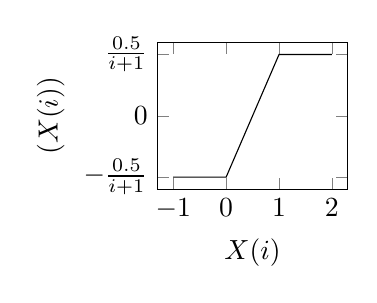
\begin{tikzpicture}[baseline=0.8cm]
    \begin{axis}[width=4cm,xlabel={$X(i)$},xtick={-1,0,1,2},ylabel={$\clipfn(X(i))$},ytick={-0.5,0,0.5},yticklabels={$-\frac{0.5}{i+1}$,$0$,$\frac{0.5}{i+1}$}]
    \addplot[mark=none,samples at={-1,0,1,2}] { min(0.5, x-0.5)-min(0,x) };
    \end{axis}
    \end{tikzpicture}\]

    Observe that $\clipfn(C_2(i)-C_1(i)+0.5)$ equals $\frac{0.5}{i+1}$ if $C_1(i)\leq C_2(i)$, and $-\frac{0.5}{i+1}$ otherwise.
    This is because the counts $C_1(i),C_2(i)$ must be integers, so if $C_1(i)\leq C_2(i)$, then $C_2(i)-C_1(i)+0.5\geq 0.5$, and the expression will evaluate to $\frac{0.5}{i+1}$. Otherwise, $C_2(i)-C_1(i)+0.5<-0.5$, and the expression will evaluate to $-\frac{0.5}{i+1}$. 

    It is straightforward, then, to use the construction for $\min$/$\max$ from above to produce a feed-forward layer that computes $\clipfn\left(C_2(i)-C_1(i)\right)$. Essentially, we use $W_1$ to compute the values (using the pre-existing values from the residual stream)

    \[\frac{0.5}{i+1}, \frac{C_2(i)-C_1(i)+0.5}{i+1}, -\frac{C_2(i)-C_1(i)+0.5}{i+1}\]
    
    Then we use $W_2$ to compute

    \[\frac{0.5}{i+1}+\ReLU\left(\frac{0.5}{i+1}-\frac{C_2(i)-C_1(i)+0.5}{i+1}\right)-\ReLU\left(\frac{0.5}{i+1}-\frac{C_2(i)-C_1(i)-0.5}{i+1}\right)\]
    which equals $\clipfn(C_2(i)-C_1(i))$ as desired.
    
    Similarly, it is straightforward to construct a feed-forward layer to compare linear combinations of count terms. That is, for disjoint sets of indices $K_1$ and $K_2$, to compute
    \[\clipfn\left(\sum_{k\in K_2} c_{k} \cdot C_k(i) -\sum_{k\in K_1} c_{k} \cdot C_k(i)\right).\]

    So we can construct a feed-forward layer $f:\R^d\to\R^d$ that computes in each dimension $i$ the following

    \[f\left(\begin{bmatrix}
        v_1\\
        v_2\\
        \vdots\\
        v_{2k_3-1}\\
        v_{2k_3}\\
        \vdots\\
        v_{d-1}\\
        v_{d}\\
    \end{bmatrix}\right) =\begin{bmatrix}
        \clipfn(v_1)\\
        \clipfn(v_2)\\
        \vdots\\
        \clipfn\left(\sum_{k\in K_2} c_{k} \cdot C_k(i) -\sum_{k\in K_1} c_{k} \cdot C_k(i)\right)\\
        \clipfn\left(\sum_{k\in K_2} c_{k} \cdot C_k(i) -\sum_{k\in K_1} c_{k} \cdot C_k(i)\right)\\
        \vdots\\
        \clipfn(v_{d-1})\\
        \clipfn(v_{d})\\
    \end{bmatrix}. \]
    
    This truncates all positive values in the residual stream at this point to be $\frac{0.5}{i+1}$ at position~$i$, and all nonpositive values to be $-\frac{0.5}{i+1}$. As a result, the next application of LayerNorm (with appropriate parameter settings) scales every single value to $\pm 1$. In particular, all previously-computed Boolean values are preserved, and the newly-computed dimensions $2k_3-1,2k$ hold the correct Boolean value based on the desired comparison